\documentclass[11pt, oneside]{article}   	% use "amsart" instead of "article" for AMSLaTeX format
\usepackage{geometry}                		% See geometry.pdf to learn the layout options. There are lots.
\geometry{letterpaper, margin=1.0in}                   		% ... or a4paper or a5paper or ... 
%\geometry{landscape}                		% Activate for rotated page geometry
\usepackage[parfill]{parskip}    		% Activate to begin paragraphs with an empty line rather than an indent
\usepackage{graphicx}				% Use pdf, png, jpg, or eps§ with pdflatex; use eps in DVI mode
								% TeX will automatically convert eps --> pdf in pdflatex		
\usepackage{amssymb}

%SetFonts

%SetFonts


\title{Circumgalactic dust halos update}
\author{Jacqueline McCleary}
%\date{}							% Activate to display a given date or no date

\begin{document}
\maketitle
\section{Overview}

Never one to give up completely, I have been pushing on this project as much as I can. Over the last year or so, here is what I have been able to do: 
\begin{enumerate}
\item Significantly refactor analysis code repository, making it more modular and robust. 
\item Weed out a few bugs in the 
\end{enumerate}
The following remains my 

\section{Code flow}
As stated above, I have endeavored to make \texttt{dusthalos} more useable and robust than it was before, incorporating use of configuration files (not hardcoded numbers) nterfacing with code via configs, separating runner scripts from class definitions, etc. Also, when creating catalogs, 

\subsection{Background catalog creation}
The basic workflow is: 
\begin{enumerate}
\item Load in the HEALpix masks of foreground and background catalogs. 
\item Keep only those objects that lie in the intersection of both HEALPix masks. 
\item If needed, join the background redshift catalog with a photometric catalog.
\item If needed, create a foreground random catalog. 
\item Save both to file.

\end{enumerate}

\subsubsection{Mask handling}

\begin{figure}
\begin{center}
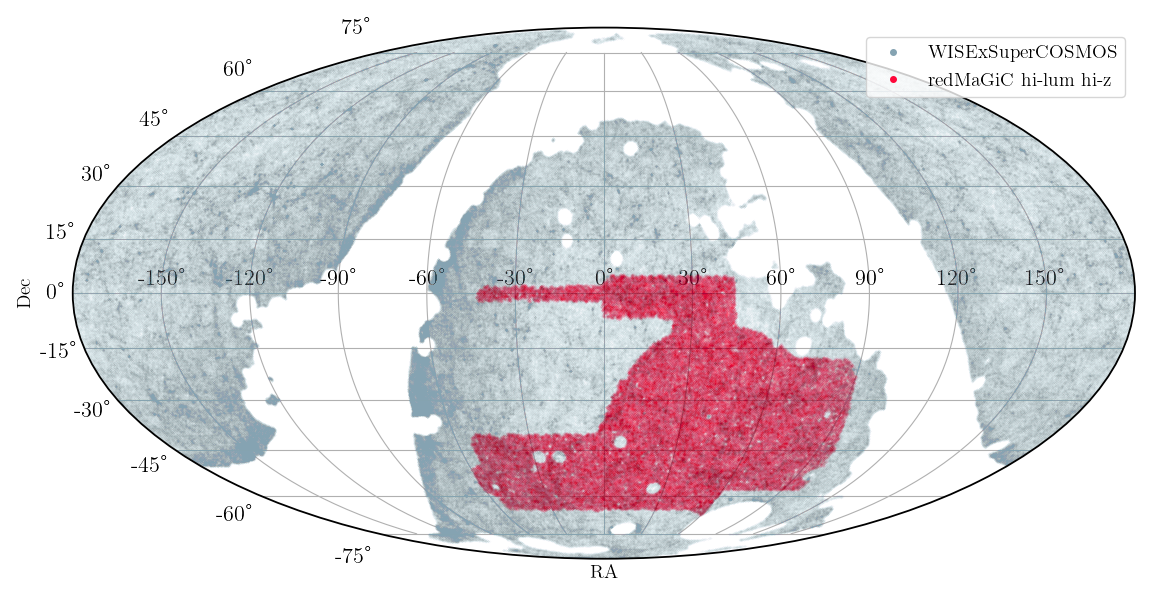
\includegraphics[width=0.65\textwidth]{figures/full_scos_hilum_hiz_overlap_mollweide_v2.png}\\
\vspace{1ex}
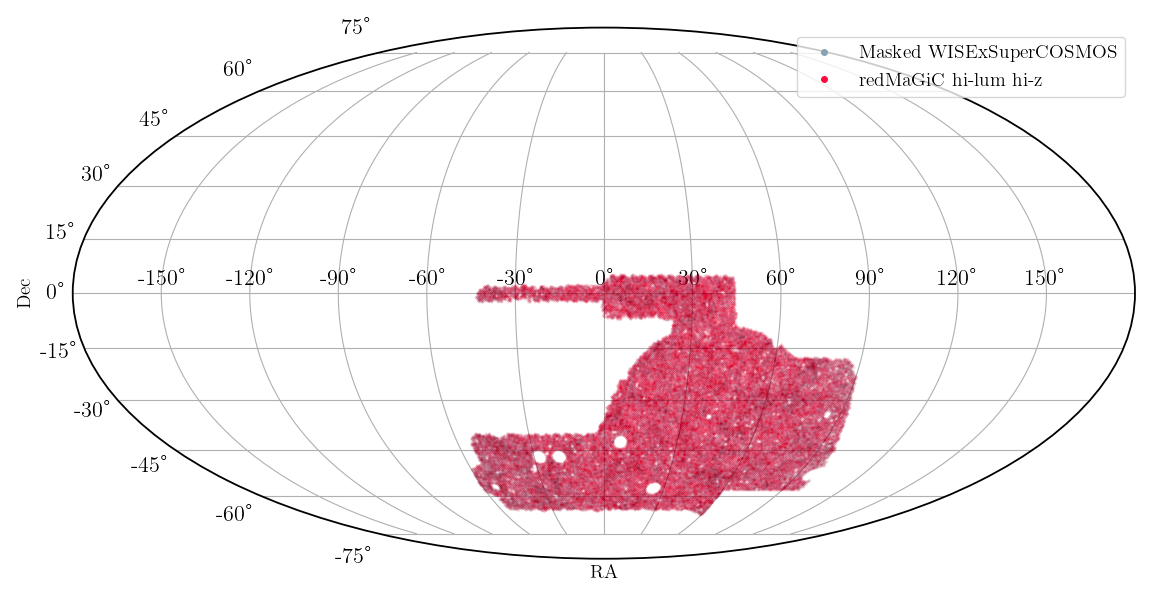
\includegraphics[width=0.65\textwidth]{figures/masked_scos_hilum_hiz_overlap_mollweide_v2.png}
\caption{Sky coverage of two catalogs used in this analysis: WISExSuperCOSMOS (foreground, grey points) and the high-luminosity high-redshift redMaGiC galaxy catalog (background, red points). The top row shows the overlap between the full WISExSuperCOSMOS catalog and the redMaGiC catalog; the bottom row shows the overlap of the two catalogs after masking.}
\label{fig:overlap1}
\end{center}
\end{figure}

\begin{figure}
\begin{center}
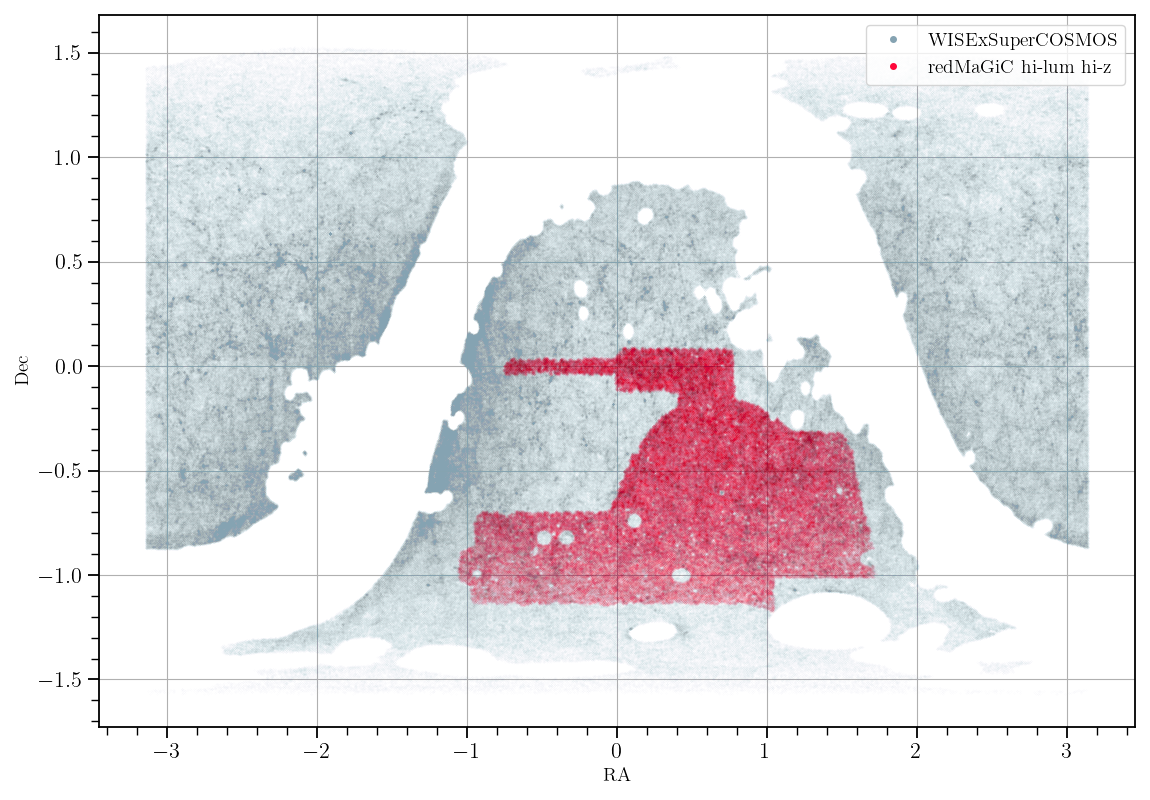
\includegraphics[width=0.49\textwidth]{figures/full_scos_hilum_hiz_overlap_rectilin.png} 
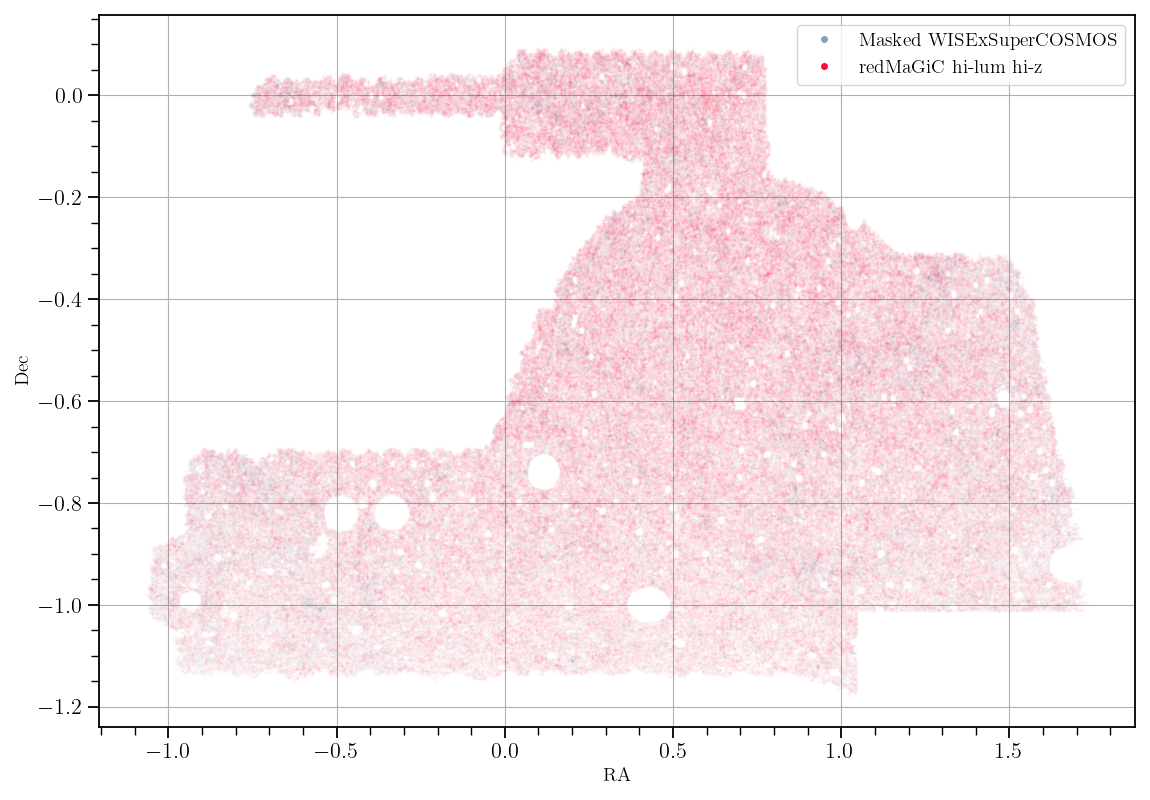
\includegraphics[width=0.49\textwidth]{figures/masked_scos_hilum_hiz_overlap_rectilin.png}
\caption{Same as Figure \ref{fig:overlap1}, but in rectilinear projection.}
\label{fig:overlap2}
\end{center}
\end{figure}


\begin{figure}
\begin{center}
\includegraphics[width=0.65\textwidth]{figures/overlap_random_rectilin.png}
\caption{Sky coverage of the WISExSuperCOSMOS random galaxy catalog generated following used in this analysis: WISExSuperCOSMOS (foreground, grey points) and the high-luminosity high-redshift redMaGiC galaxy catalog (background, red points). The top row shows the overlap between the full WISExSuperCOSMOS catalog and the redMaGiC catalog with Mollweide (left) and rectilinear (right) projections; the bottom row shows the overlap of the two catalogs after masking.}
\label{fig:overlap3}
\end{center}
\end{figure}


\subsubsection{Creating background catalogs}
The redMaGiC catalog has positions and redshifts, but not magnitudes. To obtain colors, I join them with their counterparts in the Y3 GOLD catalog on the \texttt{COADD\_OBJECT\_ID} parameter. The random galaxy catalog obviously doesn't have a corresponding entry in the GOLD catalog, so instead I match randomly.



\end{document}  